\documentclass{article}
\usepackage[utf8]{inputenc}
\usepackage[greek,english]{babel}
\usepackage{alphabeta}
\usepackage{fancyhdr}
\usepackage{listings}
\usepackage{mathtools}
\usepackage{xcolor}
\usepackage{biblatex}
\usepackage[left=2cm,right=2cm]{geometry}

\lstset {
        basicstyle=\ttfamily,
        columns=fullflexible,
        breaklines=true,
        keepspaces=true
}

\title{Σχεδίαση Ψηφιακών Συστημάτων - Εργασία Θεωρίας (Μέρος 5)}
\author{Χρήστος Μαργιώλης}
\date{Ιούλιος 2020}

\begin{document}

\begin{titlepage}
        \maketitle
\end{titlepage}

\renewcommand{\contentsname}{Περιεχόμενα}
\tableofcontents

\section{Κώδικας και τεκμηρίωση}

\subsection{\lstinline{instrmem.vhd}}

Το παρακάτω κύκλωμα υλοποιεί την μνήμη εντολών του MIPS. Ο κώδικας
είναι ίδιος με αυτόν της εκφώνησης, απλώς με λίγο διαφορετική μορφοποίηση. 
Επίσης, στην θέση μνήμης 6 έχει τοποθετηθεί και η εντολή 
\lstinline{add $4 $5 $6}. \\

\lstinputlisting[language=VHDL]{../instrmem.vhd}
\pagebreak

\subsection{\lstinline{instrmem_tb.vhd}}

Testbench για την μνήμη εντολών του MIPS. Δίνουμε διάφορες τιμές
θέσεων μνήμης και η έξοδος είναι τα περιεχόμενα της μνήμης στις θέσεις αυτές. \\

\lstinputlisting[language=VHDL]{../instrmem_tb.vhd}
\pagebreak

\subsection{\lstinline{datamem.vhd}}

Το παρακάτω κύκλωμα υλοποιεί την μνήμη εντολών του MIPS. Ο κώδικας
είναι ίδιος με αυτόν της εκφώνησης, απλώς με λίγο διαφορετική μορφοποίηση. \\

\lstinputlisting[language=VHDL]{../datamem.vhd}
\pagebreak

\subsection{\lstinline{datamem_tb.vhd}}

Testbench για την μνήμη εντολών του MIPS. Οι τιμές για το testbench πάρθηκαν
από την εκφώνηση της άσκησης. \\

\lstinputlisting[language=VHDL]{../datamem_tb.vhd}
\pagebreak

\section{Εκτέλεση}

\subsection{\lstinline{instrmem_tb}}
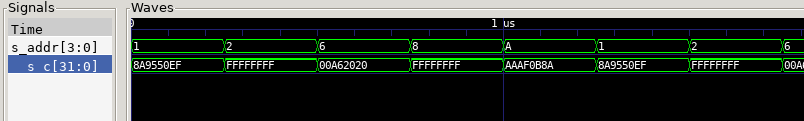
\includegraphics[width=\textwidth]{res/instrmem.png}

\subsection{\lstinline{datamem_tb}}
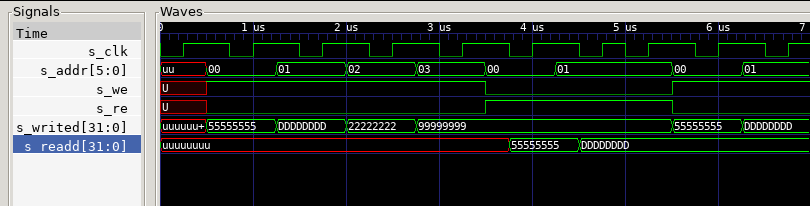
\includegraphics[width=\textwidth]{res/datamem.png}

\end{document}
